\documentclass[slide,papersize]{jsarticle}
\usepackage[dvipdfmx]{graphicx,color}
\begin{document}

\section*{WebView}
\vspace*{15mm}
\begin{center}
{\Huge {\bf WebKit の使い方}}
\end{center}

\section*{agenda}
\bigskip
\begin{itemize}
\item 簡単なサンプル
\bigskip
\item javascript の動作について
\bigskip
\item assets フォルダ
\bigskip
\item javascript との連携
\end{itemize}

\section*{簡単なサンプル}
\bigskip
\begin{itemize}
\item Manifest で permission の追加
\bigskip
\item WebView オブジェクトの生成
\bigskip
\item loadUrl
\end{itemize}

\section*{Manifest}
\begin{center}
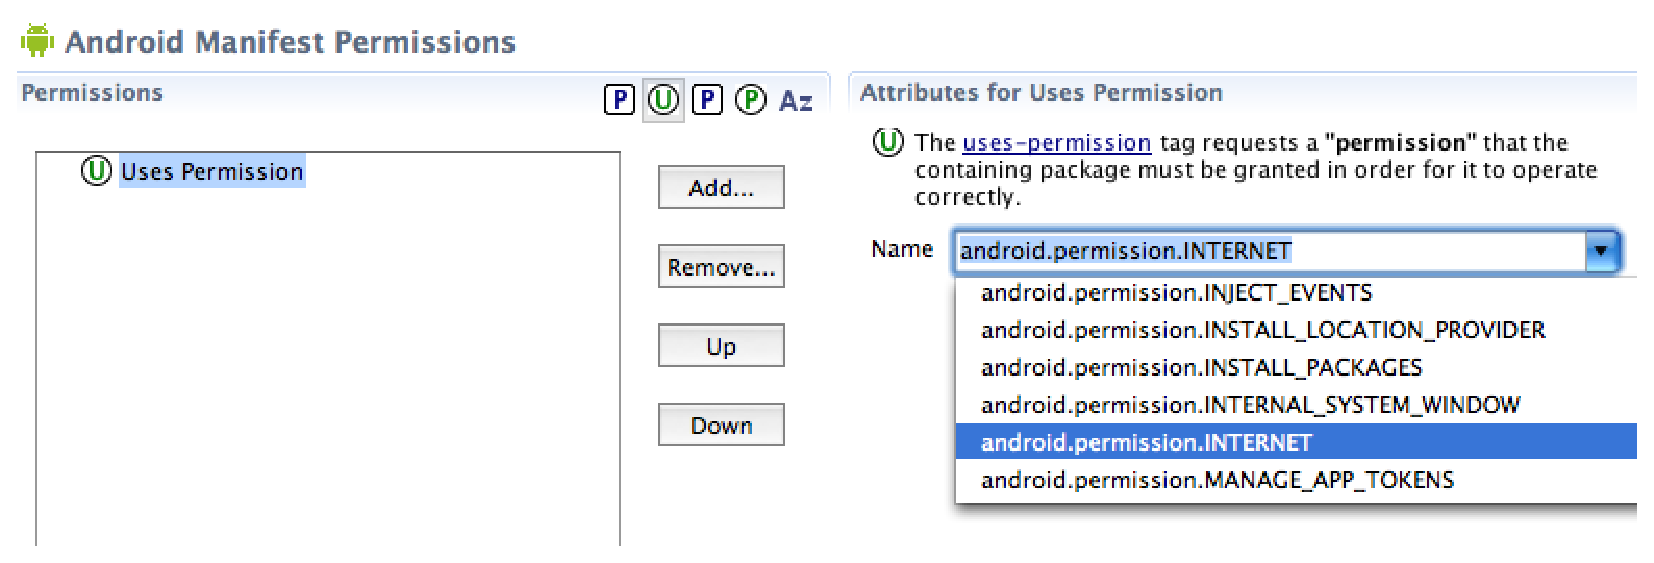
\includegraphics[scale=0.25]{internet-permission.eps}
\end{center}
インターネット接続権限の付与

\section*{Activity への盛り込み}
\begin{center}
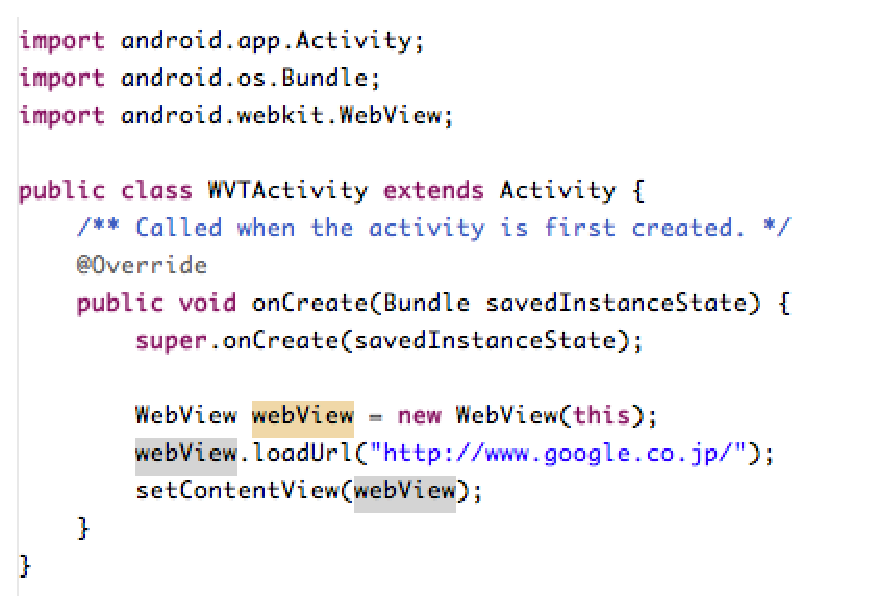
\includegraphics[scale=0.3]{WVTActivity.eps}
\end{center}
WevView オブジェクトを作って loadUrl

\section*{動かしてみよう}
\bigskip
\begin{itemize}
\item 通常のサイト表示は可能のはずです
\medskip
\item javascript を使用するサイトは?
\medskip
\item 例えば Google Maps とか
\end{itemize}

\section*{javascirpt 動作可能に}
\bigskip
\begin{center}
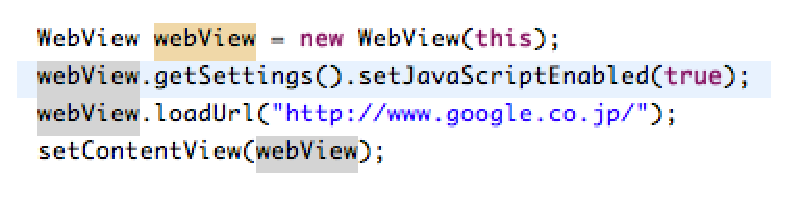
\includegraphics[scale=0.3]{javascriptEnabled.eps}
\end{center}
\begin{itemize}
\item {\footnotesize setJavaScriptEnabled メソドに true を渡します}
\item {\footnotesize Google などで確認してみましょう}
\end{itemize}

\section*{ローカルな html の処理}
\medskip
\begin{itemize}
\item ローカルな html の読み込みもできます
 \begin{itemize}
 \medskip
 \item 方法は以下
 \item {\footnotesize loadUrl(file:///android\_asset/xxx.html);"}
 \end{itemize}
\medskip
\item assets 配下にファイルを投入すれば OK
\end{itemize}
試してみましょう。

\section*{javascript との連携}
\bigskip
\begin{itemize}
\item javascript interface
\bigskip
\item サンプル以下です
\bigskip
\item http://db.tt/N5fz7L
\bigskip
\item download したファイルを展開して import
\end{itemize}

\section*{javascript}
\bigskip
\begin{itemize}
\item 基本的にはブラウザ上で非同期に動作
\bigskip
\item リアルタイムな処理には向かない
\bigskip
\item html5 + CSS + javascript の可能性
\end{itemize}

\end{document}
